 % use the "wcp" class option for workshop and conference
 % proceedings
 %\documentclass[gray]{jmlr} % test grayscale version
 %\documentclass[tablecaption=bottom]{jmlr}% journal article
 \documentclass[tablecaption=bottom,wcp]{jmlr} % W&CP article

 % The following packages will be automatically loaded:
 % amsmath, amssymb, natbib, graphicx, url, algorithm2e

 %\usepackage{rotating}% for sideways figures and tables
 %\usepackage{longtable}% for long tables

 % The booktabs package is used by this sample document
 % (it provides \toprule, \midrule and \bottomrule).
 % Remove the next line if you don't require it.
\usepackage{booktabs}
 % The siunitx package is used by this sample document
 % to align numbers in a column by their decimal point.
 % Remove the next line if you don't require it.
\usepackage[load-configurations=version-1]{siunitx} % newer version
 %\usepackage{siunitx}
 \usepackage{easyeqn}

 % The following command is just for this sample document:
\newcommand{\cs}[1]{\texttt{\char`\\#1}}% remove this in your real article

 % Define an unnumbered theorem just for this sample document for
 % illustrative purposes:
\theorembodyfont{\upshape}
\theoremheaderfont{\scshape}
\theorempostheader{:}
\theoremsep{\newline}
\newtheorem*{note}{Note}

\jmlrproceedings{Bayesian Methods of Machine Learning 2020}{Bayesian Methods of Machine Learning 2020}

 % The optional argument of \title is used in the header
\title[Project Report]{Super-Samples from Kernel Herding}

 \author{\Name{Georgii Novikov}}

\DeclareMathOperator*{\argmax}{arg\,max}
\DeclareMathOperator*{\argmin}{arg\,min}
\DeclareMathOperator{\E}{\mathop{{}\mathbb{E}}}
\DeclareMathOperator{\Var}{Var}
\newcommand\R{\mathbb{R}}
\newcommand{\norm}[1]{\left\lVert#1\right\rVert}
\newcommand{\dotprod}[2]{\langle #1, #2 \rangle}

\begin{document}

\maketitle

\begin{abstract}
Project report on reproducing the paper "Super-samples from Kernel Hearding" \cite{Chen2012} -- paper about kernel version of herding procedure, that iteratively builds a subset, empirical distribution of which approximates the true distribution, and that has a rate of convergence $\mathcal{O}(T^{-1})$.
\end{abstract}


\section{Introduction}
    The considered paper \cite{Chen2012} is a follow-up paper in the chain of several papers (\cite{Chen2010}, \cite{Welling2010}, \cite{Welling2}, \cite{Welling3}) which develop the so-called "herding" procedure. It is a method of generating pseudo-samples which resembles original data and could be used for dataset compression, estimate quantities of interest, compression of model ensembles. The key benefit of the herding procedure is that it has an $\mathcal{O}(T^{-1})$ convergence rate, which is significantly better than $\mathcal{O}(T^{-\frac{1}{2}})$ convergence rate of i.i.d samples.

    In the paper of interest, the kernel version of herding algorithm was described. Then, it was proved, that the same asymptotic guarantees still hold for the kernelized version. And then the developed procedure was tested on several model tasks.

    In this report, I first describe the herding procedure and how to obtain the kernelized version of it in section \ref{sec:theory}. Then in section \ref{sec:experiments}, I reproduce the experiments from the original paper. In section \ref{sec:discussion}, I describe my criticism regarding the paper and sum up my work done.


\section{Theory} \label{sec:theory}

    \subsection{Herding}
        Let $\set{X} \subset \R^n$ is some space with a probability distribution $p(\vec{x})$ on it, $\vec{x} \in \set{X}$ and $\vec{ \phi(\vec{x})} : \set{X} \rightarrow \set{H}$ is some feature map function to the Hilbert space $\set{H}$ with inner product $\langle \dot, \dot \rangle$. Then herding is a weakly-chaotic, non-linear dynamical system, consisted of the following update equations for a weight-vector $\vec{w} \in \set{H}$ (\cite{Chen2010}, \cite{Welling2010}):
        \begin{EQA}[l] \label{nonkernel-herding}
                \vec{x}_{t + 1} = \argmax_{\vec{x} \sim \set{X}} \langle \vec{w}_t, \vec{x} \rangle \\
                \vec{w}_{t + 1} = \vec{w}_t + \E_{\vec{x} \sim p} \left[ \vec{\phi}(\vec{x}) \right] - \vec{\phi}(\vec{x}).
        \end{EQA}
        For easy of intuitive understanding of herding, under some assumptions, the iterative procedure \eqref{nonkernel-herding} could be viewed as a greedy optimization of the squared error $\varepsilon_T^2$ defined as
        \begin{EQA}[l] \label{nonkernel-error}
            \varepsilon_T^2 = \norm{\mu_p - \frac{1}{T} \sum_{t=1}^T \vec{\phi}(\vec{x})}^2,
        \end{EQA}
        where $\mu_p = \E_{\vec{x} \sim p} \vec{\phi}(\vec{x})$. The key result about herding is that if we manage to find optimal $\vec{x}_t$ on each iteration of \eqref{nonkernel-herding}, then the error in \eqref{nonkernel-error} decreases at a rate of $\mathcal{O}(T^{-1})$. It is a very nice result, because, for instance, randomly generated i.i.d samples would have a $\mathcal{O}(T^{-1})$ rate of convergence, and samples, produced by MCMC, would have positive autocorrelation and thus have even worse rate of convergence.

    \subsection{Kernel Trick}
        In order to apply herding procedure \eqref{nonkernel-herding}, we have to store state vector $\vec{w}$ explicitly, which means, that we can not work in an infinite-dimensional Hilbert space. To overcome this, we can make a standard kernel trick: substitute explicit function $\vec{\phi(\vec{x})}$ with an implicit one, given by the kernel function $k(\vec{x}, \vec{x}') = \langle \vec{\phi}(\vec{x}), \vec{\phi}(\vec{x}') \rangle$. Making an assumption, that $\vec{w}_0 = \mu_p$, we can rewrite \eqref{nonkernel-herding} in the following way:
        \begin{EQA}[rcl] \label{kernel-herding}
            \vec{x}_{T + 1}
            & = & \argmax_{\vec{x} \in \set{X}} \dotprod{\vec{w}_0}{\vec{\phi}(\vec{x})} + T \E_{\vec{x}' \sim p} \left[ k(\vec{x}, \vec{x}') \right] - \sum_{t=1}^{T} k(\vec{x}, \vec{x_t}) \\
            & = & \argmax_{\vec{x} \in \set{X}} \E_{\vec{x}' \sim p} - \frac{1}{T + 1} \sum_{t=1}^{T} k(\vec{x}, \vec{x}').
        \end{EQA}
        It can be shown, that kernel herding is performing greedy minimization of
        \begin{EQA}[rcl] \label{kernel-error}
            \varepsilon_T^2 & = & \norm{\mu_p - \frac{1}{T} \sum_{t=1}^T \vec{\phi}(\vec{x})}^2 \\
                            & = & \E_{\vec{x}, \vec{x}' \sim p} \left[ k(\vec{x}, \vec{x'}) \right] - \frac{2}{T} \sum_{t=1}^{T} \E_{\vec{x} \sim p} k(\vec{x}, \vec{x_t}) + \frac{1}{T^2} \sum_{t, t' = 1}^{T} k(\vec{x}_t, \vec{x}_{t'}).
        \end{EQA}
        The error measures the distance between $p$ and the empirical distribution $\hat{p}_T(\vec{x}) = \frac{1}{T} \sum_{t=1}^{T} \delta(\vec{x}, \vec{x}')$, and the kernel $k(\vec{x}, \vec{x}')$ determines how we should measure distances between distributions. The central result of the observed paper is that kernel herding still has $\mathcal{O}(T^{-1})$ rate of convergence.


\section{Experiments} \label{sec:experiments}

    \subsection{Toy example} \label{subsec:toy}
        To begin with, authors show how herding works on a toy 2D mixture of Gaussians. On a Figure \ref{fig:toy} you can see the difference between first 20 herded samples and 20 i.i.d samples. All modes are getting attentions and samples are distributed overall in a "pleasant way".

        \begin{figure}
            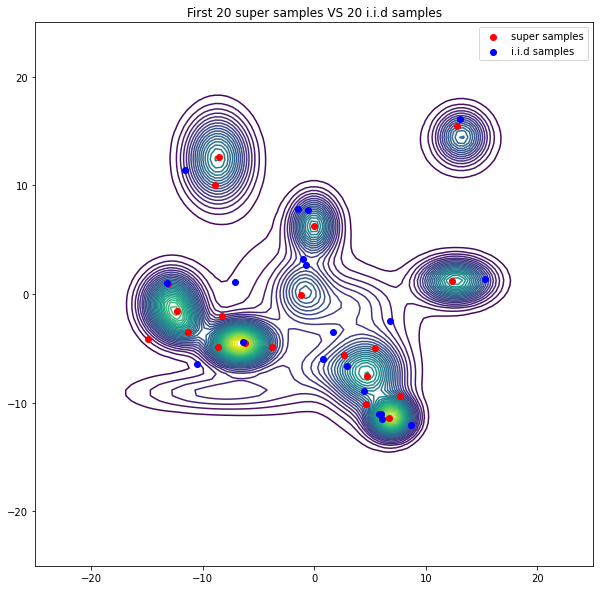
\includegraphics[width=\textwidth]{images/toy}
            \caption{Comparision of 20 super-samples (obtained by herding) and 20 i.i.d samples for mixture of 10 2-dimensional Gaussians}
            \label{fig:toy}
        \end{figure}

    \subsection{Matching the True Distribution} \label{subsec:true}
        A mixture of 100 5-dimensional Gaussian distributions was generated. Error was computed on four functions: the first three moments, and a non-linear function. Firstly average value of $f(x_{i, t})$ was calculated (where $f(x) = x^m, m = 1, 2, 3$ for moments and $f(x) = \sin(x)$ for sine function) and then the RMSE of the estimated value  was computed:
        \begin{EQA}[l] \label{approx_error}
            err(\set{S}_T) = \left( \frac{1}{d} \sum_{i=1}^{d} \left( \langle f(x_i) \rangle_{\set{s}_T} - \langle f(x_i) \rangle_{p} \right)^2 \right).
        \end{EQA}
        The results are shown on the Figure \ref{fig:true}.

        \begin{figure}
            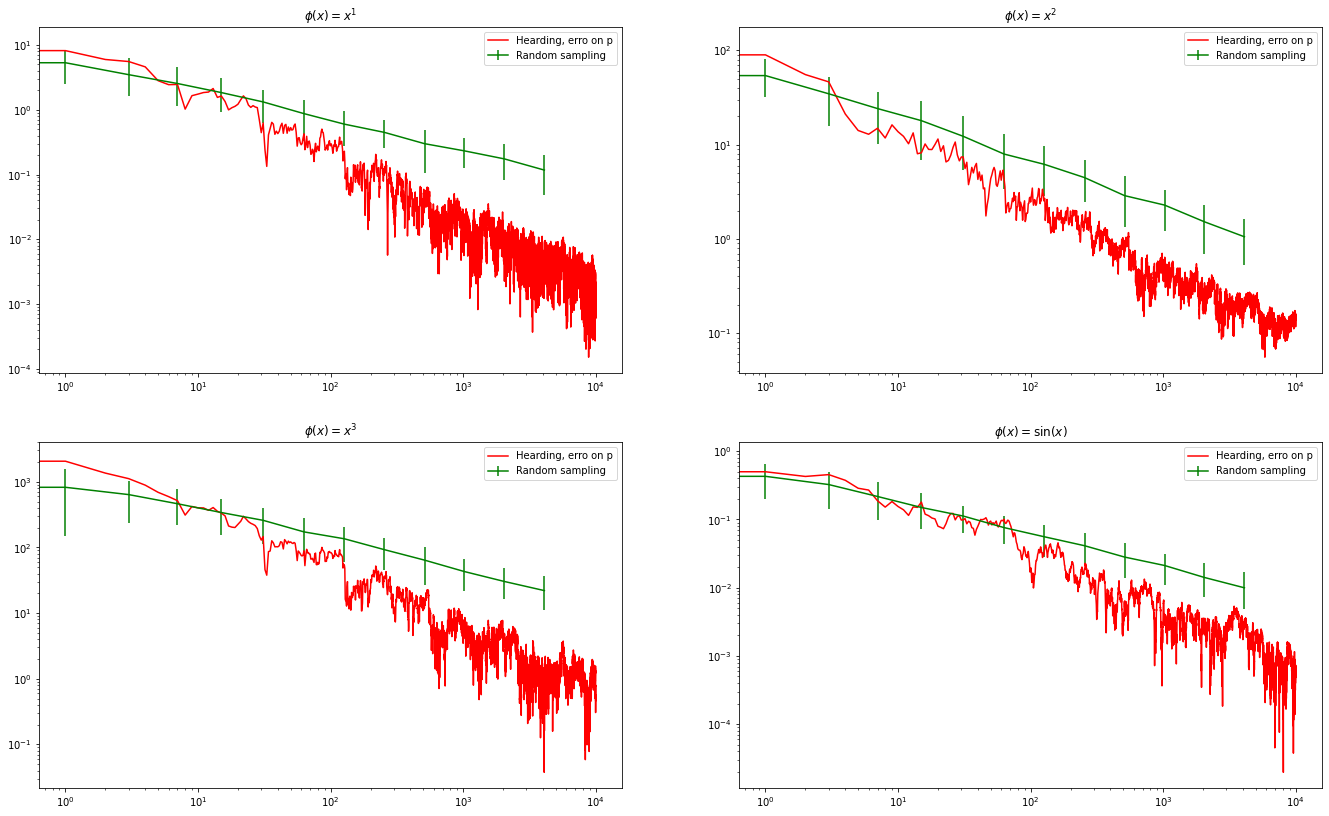
\includegraphics[width=\textwidth]{images/true}
            \caption{Dependence of approximation error \eqref{approx_error} on the number of samples for Gaussian Mixture. Red line is samples acquired by herding. Green line is i.i.d samples from mixture.}
            \label{fig:true}
        \end{figure}

    \subsection{Matching Empirical Distribution} \label{subsec:empirical}
        The expectation in \eqref{kernel-herding} can not be computed explicitly in the general case. But if we  have a set $\set{D}$ of i.i.d samples from the distribution, we can run herding to match the empirical distribution. A set of $10^5$ samples is drawn from the mixture and then used as a true distribution for herding. In this case expectation in \eqref{kernel-herding} is just an average over all samples. The estimation of function is again compared between herding and random samples. On Figure \ref{fig:empirical} we can see, that only a couple of thousands super samples is required to achieve similar approximation quality of the true mixture quantity.

        \begin{figure}
            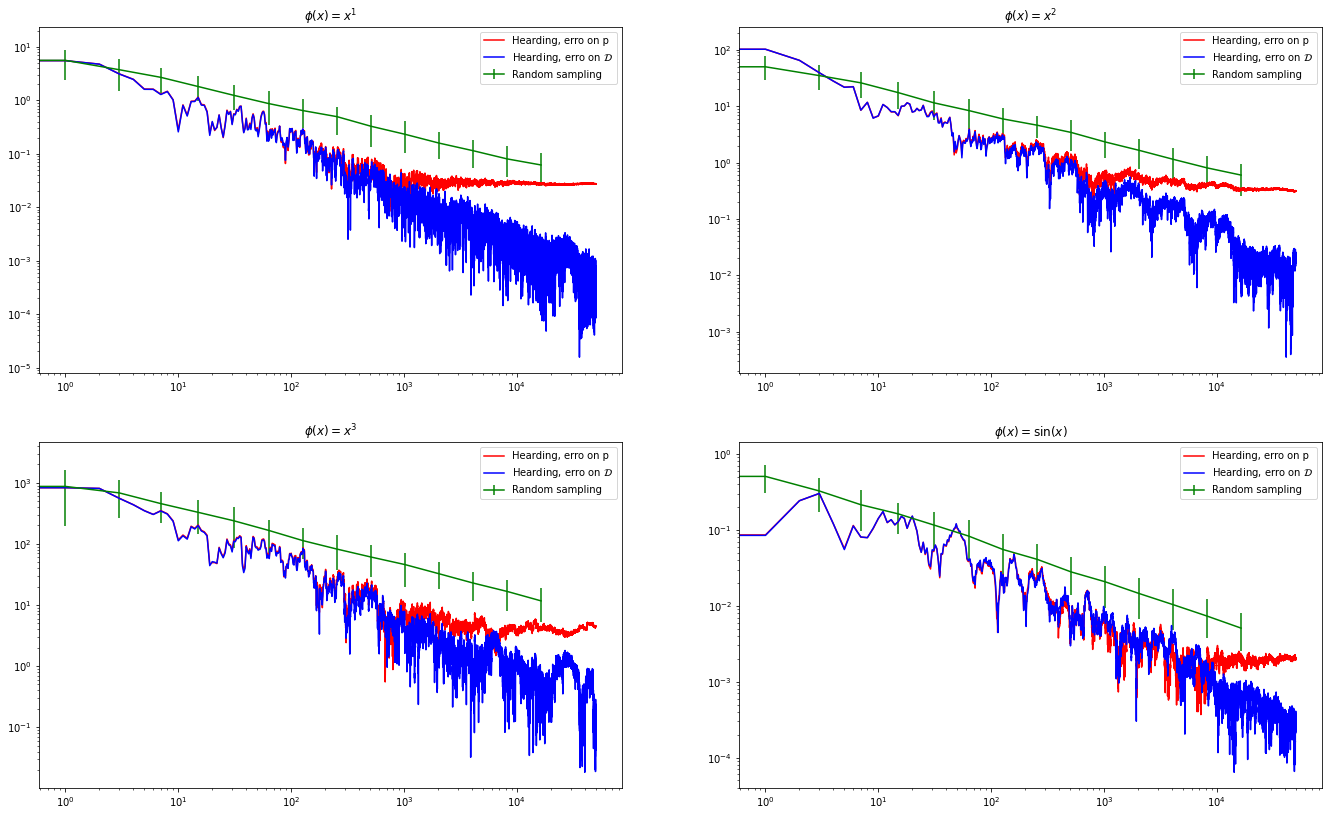
\includegraphics[width=\textwidth]{images/empirical}
            \caption{Dependence of approximation error \eqref{approx_error} on the number of samples for Gaussian Mixture in the empirical distribution matching setup. Red and blue lines are samples acquired by herding for the approximating true value (red) and empirical value (blue). As the empirical value goes to the zero with an increasing number of herded elements, red line stagnates on several thousands (as we can not approximate better than the initial sample pool $\set{D}$. Which means, that we can significantly compress the dataset $\set{D}$ without huge quality loss. Green line is i.i.d samples from mixture (measured on true distribution).}
            \label{fig:empirical}
        \end{figure}


    \subsection{Approximating the Bayesian Posterior} \label{subsec:bayes}
        The final experiment in the original paper is an approximating the predictive distribution of a Bayesian model. Authors took the UCI spambase dataset that has 4601 instances (which were split into 3000 instances for train and 1601 for test) with 57 real attributes and 1 binary class label. The training set was whitened by a PCA and then fed into logistic regression model with Gaussian prior to draw a set of $10^7$ samples by Metropolis-Hasting procedure with Gaussian proposal distribution. And the resulting set was subsampled by a factor of $100$ to reduce the autocorrelation. This set $\set{D}$ was whitened with PCA and fed into herding procedure with an isotropic Gaussian kernel with $\sigma = 10$. The quality of the resulting set $\set{S}_T$ of supersamples was tested with the following error:
        \begin{EQA}[l]
            \text{RMSE}^2(\set{S}_T, \set{D}) = \frac{1}{N} \sum_{n=1}^{N} \left[ \frac{1}{T} \sum_{t=1}^{T} p(y_n | x_n, \theta_t) - \frac{1}{|D|} \sum_{d=1}^{|D|} p(y_n | x_n, \theta_d) \right]^2
        \end{EQA}
        For comparision, random samples was drawn from $\set{D}$ by bootstrapping and computed error in the same way to model the performance of the i.i.d samples. Also, the much larger set of $2.5 * 10^6$ posterior samples were drawn in the same way as $\set{D}$ to estimate the error of $\set{S}_T$ on $p$ by $\text{RMSE}(\set{S}, p)$ (the red line on Figure \ref{fig:bayes}). With that we can see that a couple of thousands of super-samples are enough to achieve similar predictive distribution approximation quality.

        \begin{figure}
            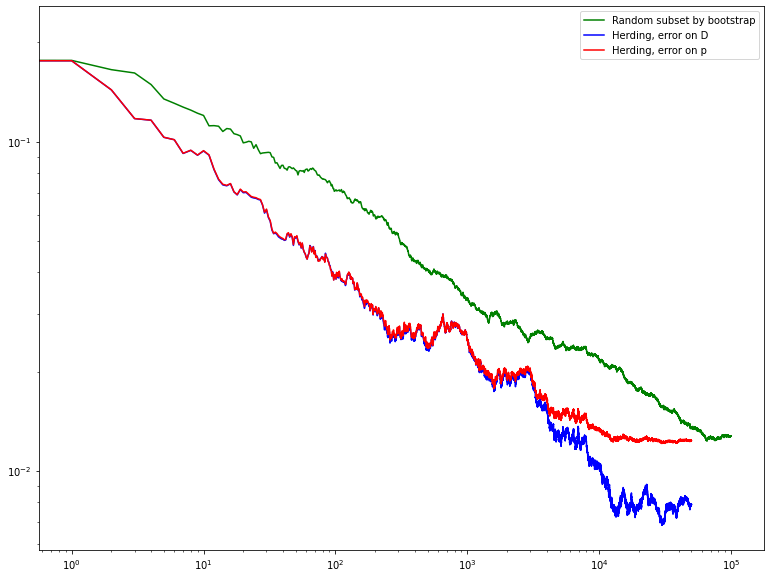
\includegraphics[width=.8\textwidth]{images/bayes}
            \caption{RMSE of the predicted probability of herding (blue - measured with respect to $\set{D}$, red - measured with respect to much larger set, which imitates the true distribution $p$) and a random subset (green)}
            \label{fig:bayes}
        \end{figure}

\section{Discussion} \label{sec:discussion}
    In this project I was managed to successfully reproduce all the experiments, that was presented by the authors in the original paper. All pictures in this report are plotted by me, the code for exact reproduction could be found in the jupyter notebook file in \href{https://github.com/PgLoLo/kernel-herding}{https://github.com/PgLoLo/kernel-herding}.

    Paper does not contain all the required information: a lot of small details are missing: parameters of Gaussian Mixtures, an exact algorithm of generating mixtures, parameters of Gaussian kernels for kernel herding, parameters of logistic regression prior and exact Metropolis-Hasting proposal distribution. But anyway, pretty much everything was reproducible with some guessing involved.

    An important moment, about which I did not manage to find information in the paper is the dependence on the hyperparameters of the kernel for kernel herding. Namely, it turned out, that the scale of the Gaussian kernel has a great influence on the resulting graphics of the approximation quality. On the Figure \ref{fig:counterpart} you can see the counterpart of the Figure \ref{fig:empirical} -- the repetition of the same empirical distribution matching experiment, but with Gaussian kernel with $\sigma = 1$. As you can see, we do not see the same superiority of herding over i.i.d samples. That fact added difficulties to the reproduction of the paper, but with trial and error everything worked out in the end.

    \begin{figure}
        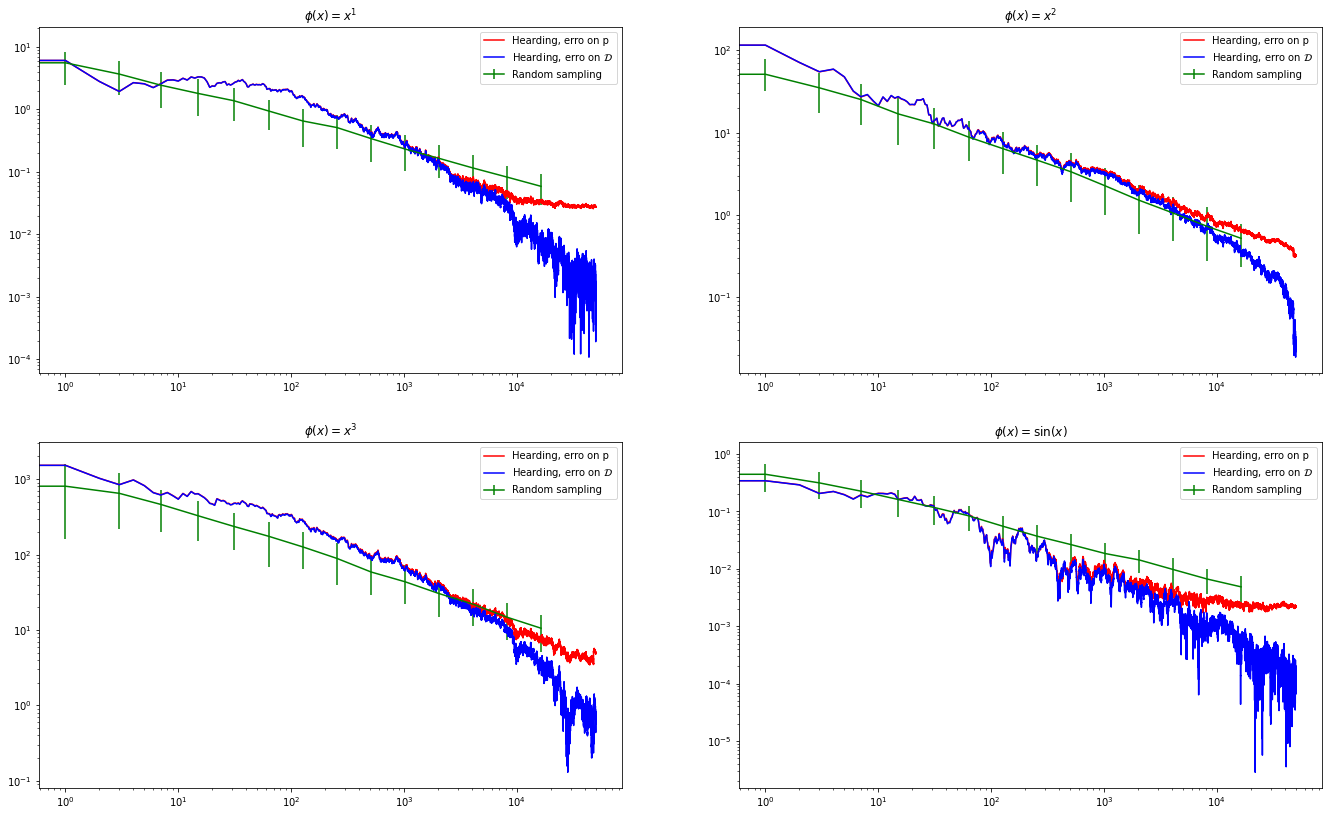
\includegraphics[width=.8\textwidth]{images/counterpart}
        \caption{Repeated matching empirical distribution experiment (section \ref{subsec:empirical} and Figure \ref{fig:empirical}) with Gaussian kernel with $\sigma = 1$.}
        \label{fig:counterpart}
    \end{figure}

% \printbibliography

\bibliography{refs}

\end{document}
